\documentclass{paper}


\usepackage{epsfig}
\usepackage{graphicx}
\usepackage{amsmath}
\usepackage{amssymb}
\usepackage{amsthm}

\usepackage{color}
\usepackage{subcaption}
\usepackage{caption}




\usepackage{mathrsfs}
\usepackage{algpseudocode}
\usepackage{algorithm}

\usepackage{float}
\usepackage{mathtools}
\usepackage{mdwlist}
\usepackage{gensymb}
\usepackage{array}
\usepackage{multirow}
\usepackage[hmargin=3cm]{geometry}
\usepackage{boxedminipage}
\usepackage{enumerate}


\setlength{\parindent}{0pt}
\setlength{\parskip}{18pt}


\usepackage[latin1]{inputenc} 
\usepackage[T1]{fontenc} 

\usepackage{listings} 
\lstset{% 
   language=Matlab, 
   basicstyle=\small\ttfamily, 
} 






\renewcommand{\algorithmicforall}{\textbf{Foreach}}
\newcommand{\init}{\textbf{INIT }}
\newcommand{\pluseq}{\mathrel{+}=}
\newcommand{\asteq}{\mathrel{*}=}
\newcommand{\myto}{\textbf{TO }}
\newcommand*\colvec[3][]{
    \begin{pmatrix}\ifx\relax#1\relax\else#1\\\fi#2\\#3\end{pmatrix}
}
\newcommand{\myparagraph}[1]{\paragraph{#1}\mbox{}\\}
\DeclarePairedDelimiter\ceil{\lceil}{\rceil}
\DeclarePairedDelimiter\floor{\lfloor}{\rfloor}



\title{Computational Photography Assignment 4}



\author{Single Michael\\08-917-445}
% //////////////////////////////////////////////////


\begin{document}



\maketitle


\section{Poisson Solver}

The following examples of \emph{Seamless Cloning}, \emph{Gradient Mixing} and \emph{Highlight Removal} are based on the so called \emph{Poisson equation} using a different gradient field. \\

In order to run a Matlab demo of these examples, please run the script \emph{start4.m} from my submitted source code. \\

All the images (and also some more), can be found in the folder \emph{outputs} in the zip file that contains my submitted Matlab code for this Project. \\

You can find the implementation of my Poisson solver in the Matlab file \emph{poissonSolver.m}.

\subsection{Seamless Cloning}

The gradient field of a certain region (determined by a mask) in a given target image is supposed to be replaced by the (masked) gradient field from a source image. The task is to fit the source gradient field to the gradient field of the target image at the masked location in the image. \\

For this task I have implemented three examples shown below. \\

You can find the implementation of my Seamless Cloning driver in the Matlab file \emph{seamlessCloning.m}.

% input
\subsubsection{Map Example}
\begin{figure}[H]
    \centering
    \begin{subfigure}{1.0\textwidth}
        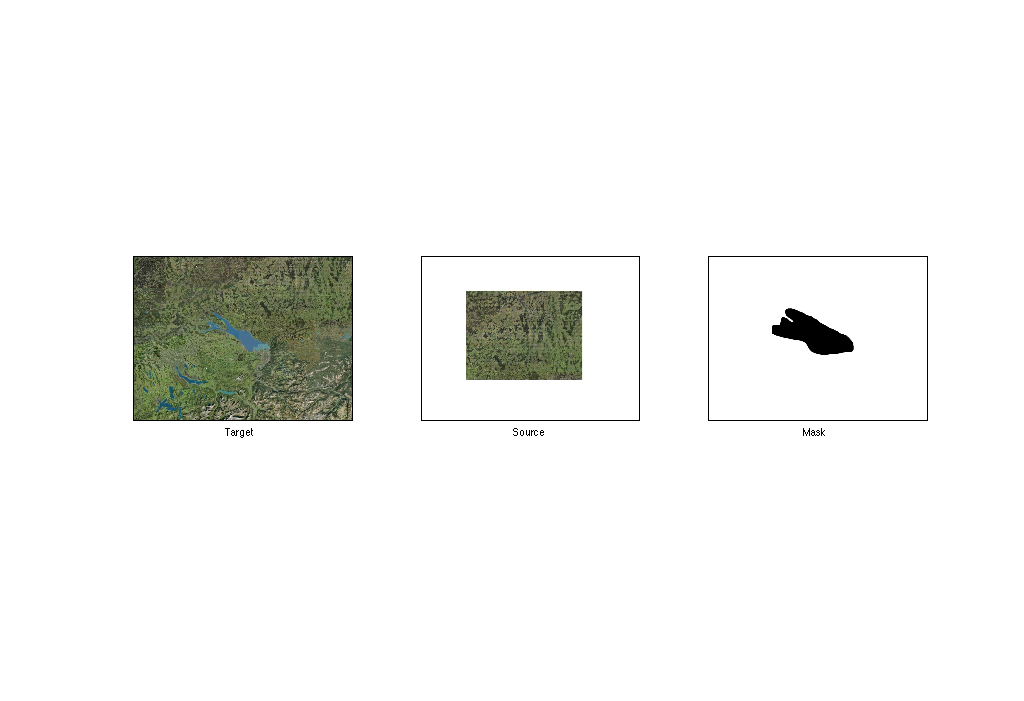
\includegraphics[width=\textwidth]{../../outputs/p4/seamless_cloning/map/input}
    \end{subfigure}
    \caption{Visualization of Input images: Target Image is a texture map (legt), the source image is a patch of another map (center), and the corresponding mask (right)  is a sub-selection of the source patch-map.}
    \label{fig:seamless_cloning_map_input}       
\end{figure}


\begin{figure}[H]
    \centering
    \begin{subfigure}{1.0\textwidth}
        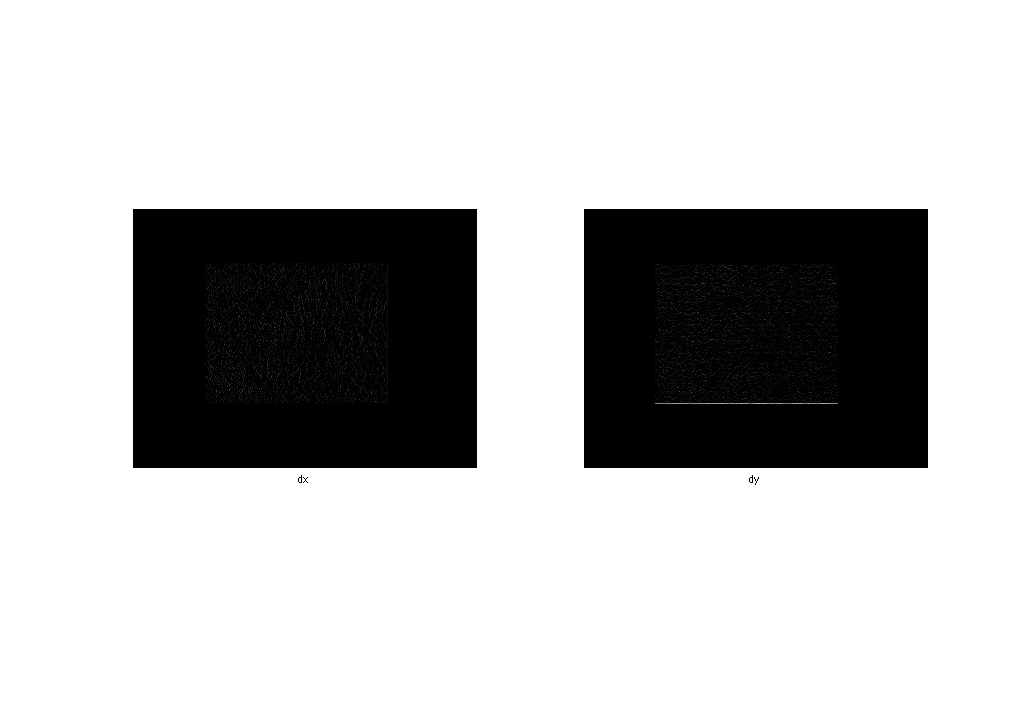
\includegraphics[width=\textwidth]{../../outputs/p4/seamless_cloning/map/gradients}
    \end{subfigure}
    \caption{Visualization of Gradient field along $dx$ and $dy$ resulting from the gradient mixing gradient field applied on each color channel encoded as an RGB image.}
    \label{fig:seamless_cloning_map_gradients}       
\end{figure}


\begin{figure}[H]
    \centering
    \begin{subfigure}{1.0\textwidth}
        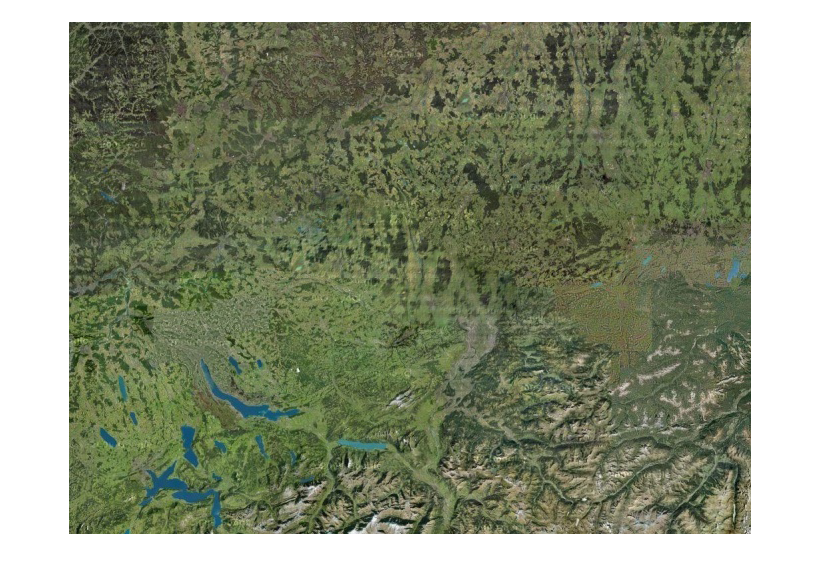
\includegraphics[width=\textwidth]{../../outputs/p4/seamless_cloning/map/output}
    \end{subfigure}
    \caption{Output resulting from the seamless cloning method applied on our given input images using the gradient field as shown above.}
    \label{fig:seamless_cloning_map_out}       
\end{figure}

\subsubsection{Plane Example}
\begin{figure}[H]
    \centering
    \begin{subfigure}{1.0\textwidth}
        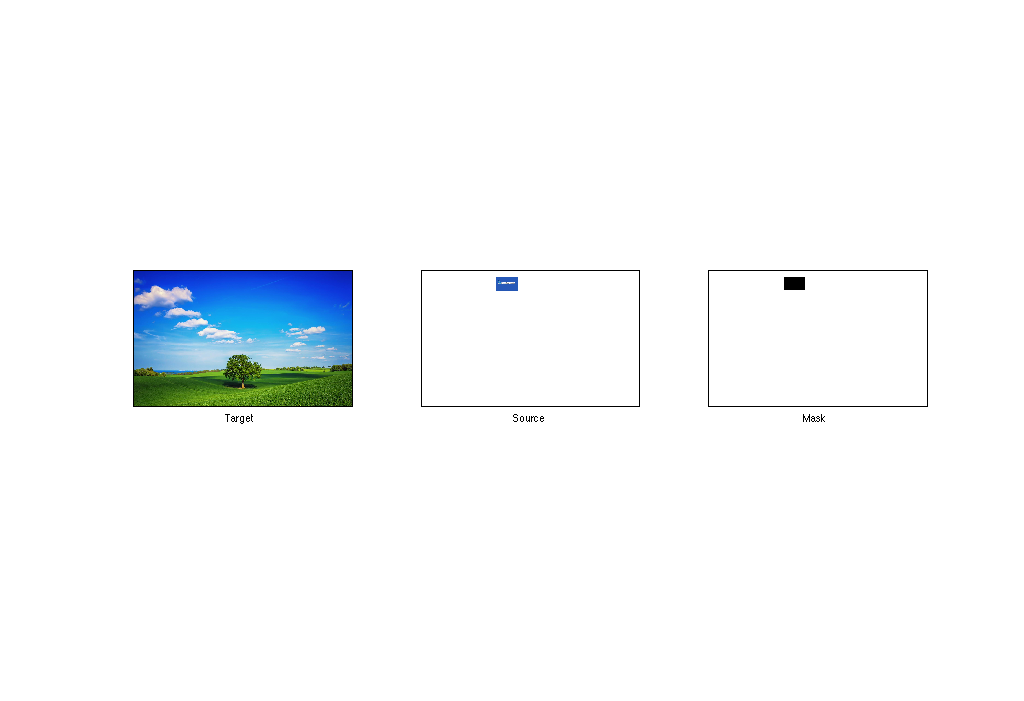
\includegraphics[width=\textwidth]{../../outputs/p4/seamless_cloning/plane/input}
    \end{subfigure}
    \caption{Visualization of Input images: Target Image illustrates a landscape (left), is an image of a plane (center), and the corresponding mask (right) is a box capturing the whole plane image.}
    \label{fig:seamless_cloning_plane_input}       
\end{figure}


\begin{figure}[H]
    \centering
    \begin{subfigure}{1.0\textwidth}
        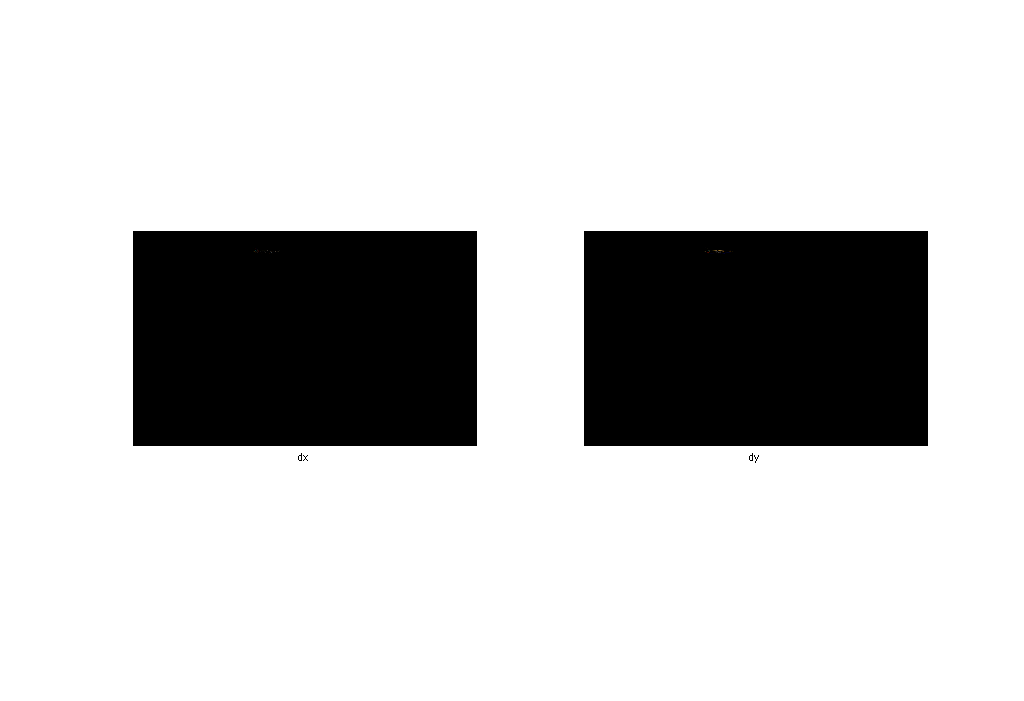
\includegraphics[width=\textwidth]{../../outputs/p4/seamless_cloning/plane/gradients}
    \end{subfigure}
    \caption{Visualization of Gradient field along $dx$ and $dy$ resulting from the gradient mixing gradient field applied on each color channel encoded as RGB images.}
    \label{fig:seamless_cloning_plane_gradients}       
\end{figure}


\begin{figure}[H]
    \centering
    \begin{subfigure}{1.0\textwidth}
        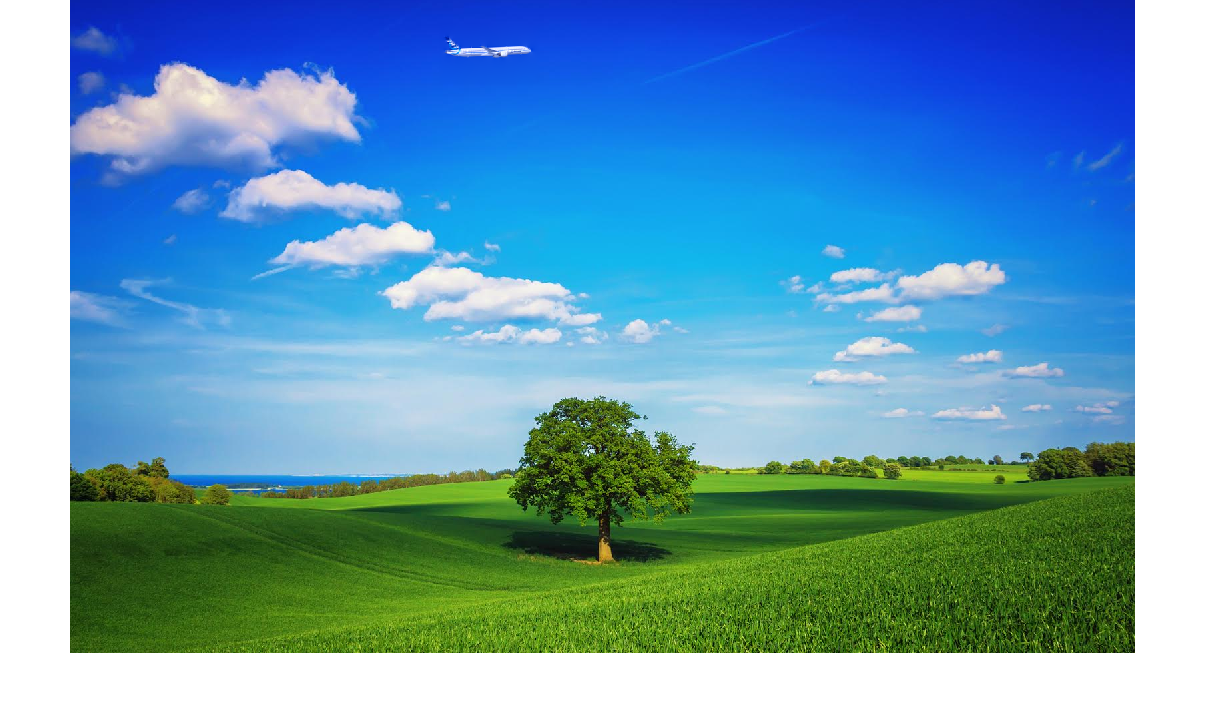
\includegraphics[width=\textwidth]{../../outputs/p4/seamless_cloning/plane/output}
    \end{subfigure}
    \caption{Output resulting from the seamless cloning method applied on our given input images using the gradient field as shown above.}
    \label{fig:seamless_cloning_plane_out}       
\end{figure}

\subsubsection{Monster Example}
\begin{figure}[H]
    \centering
    \begin{subfigure}{1.0\textwidth}
        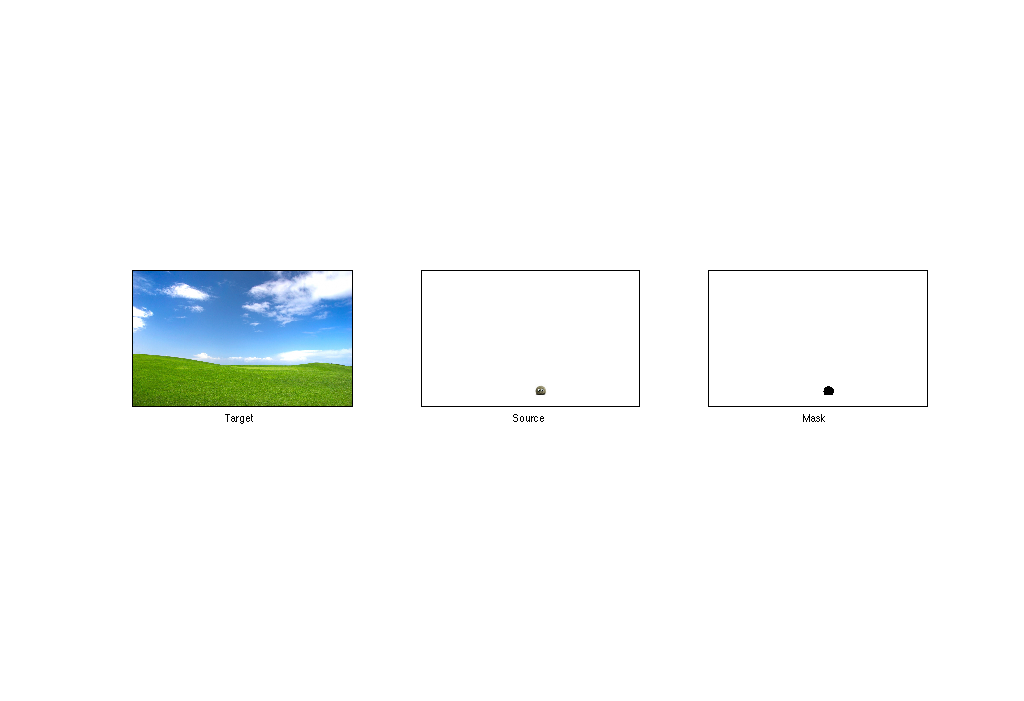
\includegraphics[width=\textwidth]{../../outputs/p4/seamless_cloning/monster/input}
    \end{subfigure}
    \caption{Visualization of Input images: Target Image is again a hilly grass landscape (left), the source image is a hairy monster (center), and the corresponding mask (right) is the contour of the monster.}
    \label{fig:seamless_cloning_monster_input}       
\end{figure}


\begin{figure}[H]
    \centering
    \begin{subfigure}{1.0\textwidth}
        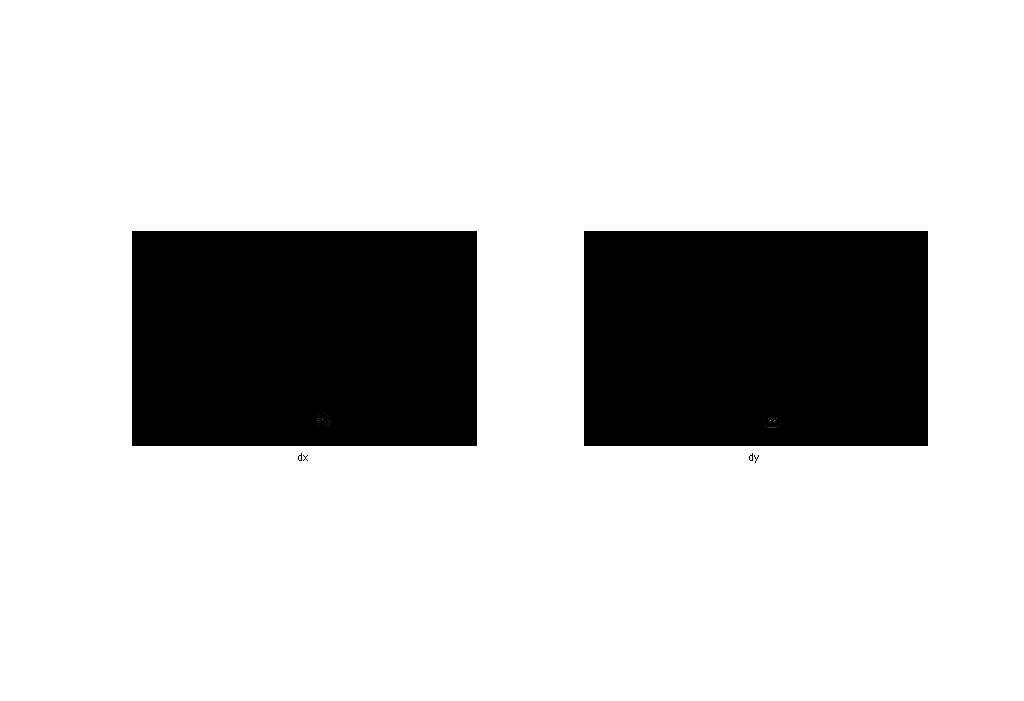
\includegraphics[width=\textwidth]{../../outputs/p4/seamless_cloning/monster/gradients}
    \end{subfigure}
    \caption{Visualization of Gradient field along $dx$ and $dy$ resulting from the gradient mixing gradient field applied on each color channel encoded in RGB images.}
    \label{fig:seamless_cloning_monster_gradients}       
\end{figure}


\begin{figure}[H]
    \centering
    \begin{subfigure}{1.0\textwidth}
        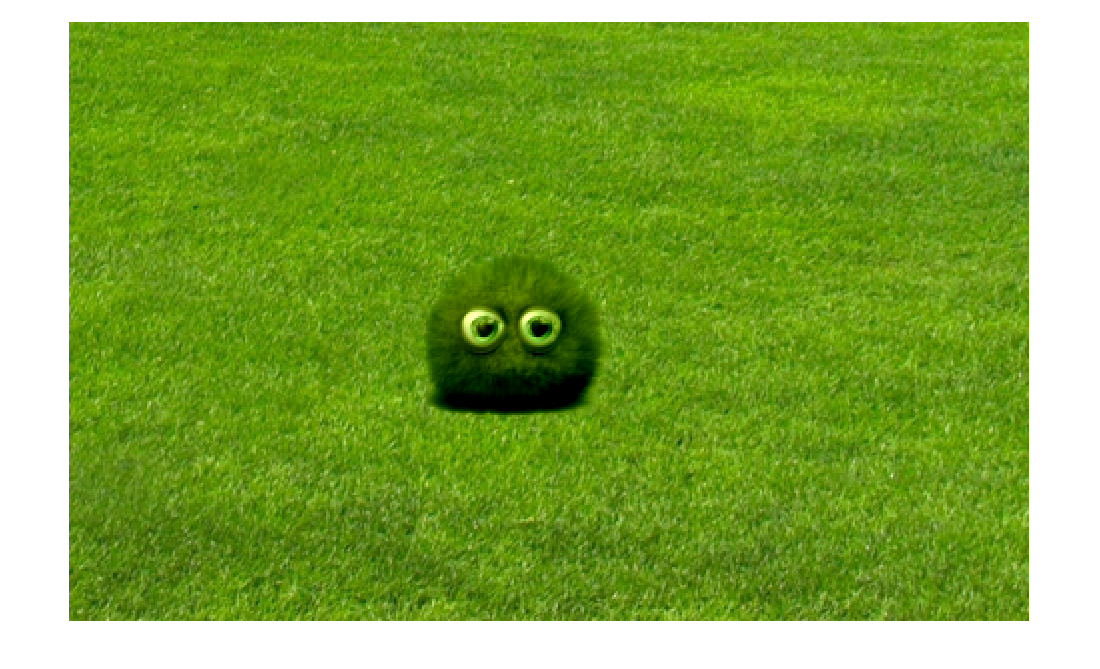
\includegraphics[width=\textwidth]{../../outputs/p4/seamless_cloning/monster/output}
    \end{subfigure}
    \caption{Output resulting from the seamless cloning method applied on our given input images using the gradient field as shown above.}
    \label{fig:seamless_cloning_monster_out}       
\end{figure}


\subsection{Gradient Mixing}

In this experiment we are interested in combining two images: One that is supposed to depict a foreground - usually a texture - and another image acting as the background image supposed to enhance some details in the given image. The method of gradient mixing will combine the gradient fields of the two images by selecting the gradient with the larger magnitude at each pixel. This will give us an output image having an additional detail layer following the gradient of the target image. Results are shown below. \\

You can find the implementation of my Seamless Cloning driver in the Matlab file \emph{gradientMixing.m}.

\begin{figure}[H]
    \centering
    \begin{subfigure}{1.0\textwidth}
        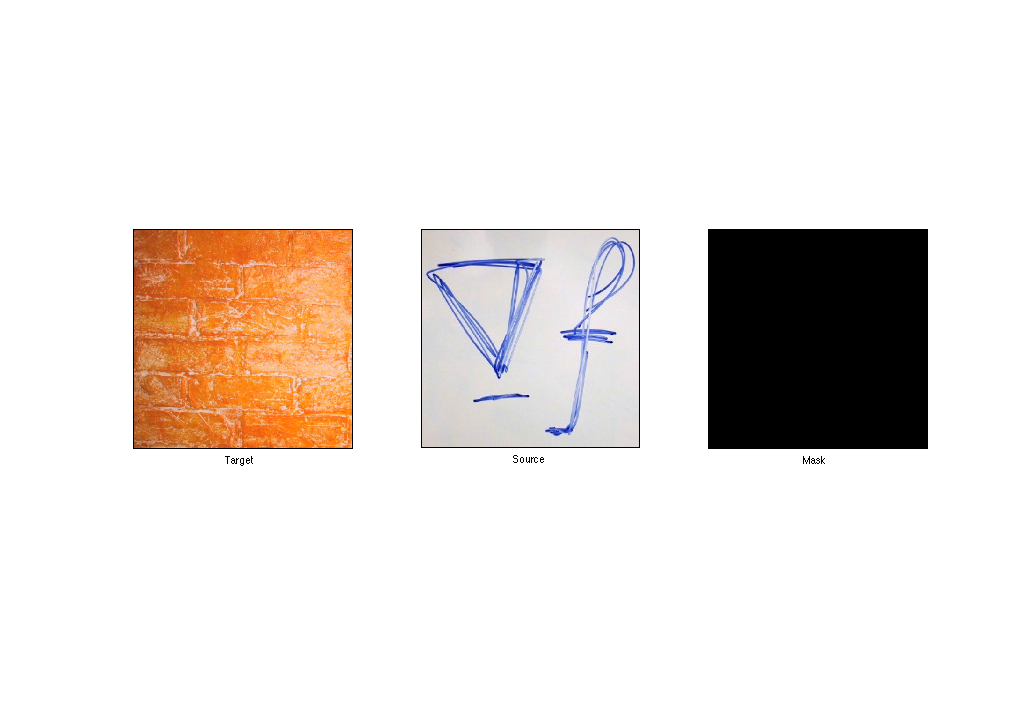
\includegraphics[width=\textwidth]{../../outputs/p4/gradient_mixing/input}
    \end{subfigure}
    \caption{Visualization of Input images: Target Image is a texture of a Wall (left), the source image is a mathematical scribble (center), and the corresponding mask (right) having a border of value one (known pixels) and everywhere else it is equal to zero.}
    \label{fig:gradient_mixing_input}       
\end{figure}


\begin{figure}[H]
    \centering
    \begin{subfigure}{1.0\textwidth}
        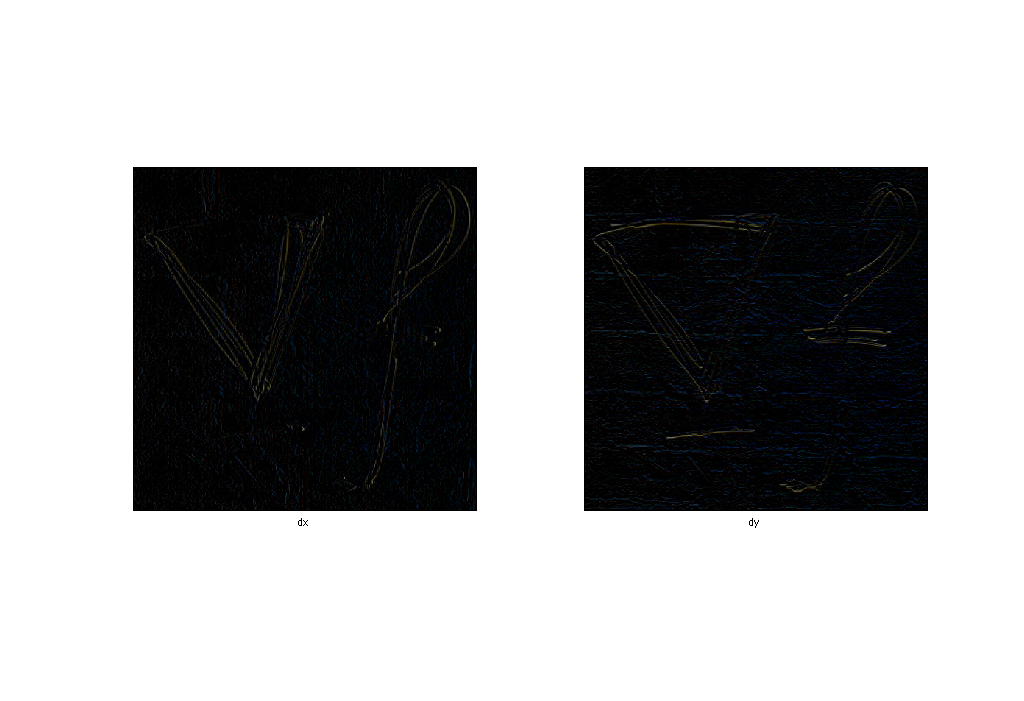
\includegraphics[width=\textwidth]{../../outputs/p4/gradient_mixing/gradients}
    \end{subfigure}
    \caption{Visualization of Gradient field along $dx$ and $dy$ resulting from the gradient mixing gradient field applied on each color channel encoded in RGB images.}
    \label{fig:gradient_mixing_gradients}       
\end{figure}


\begin{figure}[H]
    \centering
    \begin{subfigure}{1.0\textwidth}
        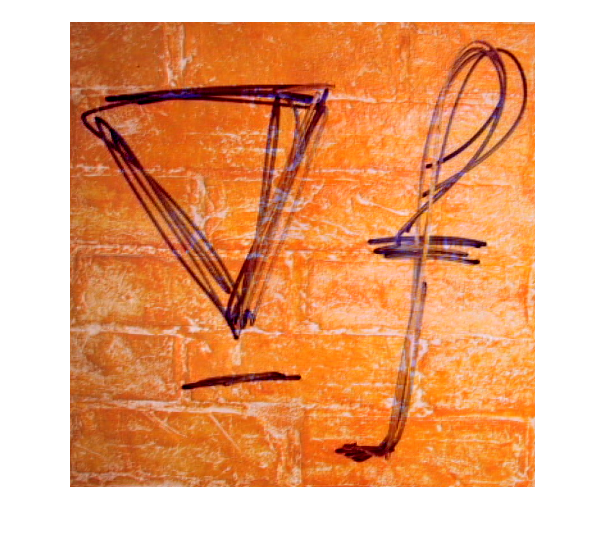
\includegraphics[width=\textwidth]{../../outputs/p4/gradient_mixing/output}
    \end{subfigure}
    \caption{Output resulting from the gradient mixing method applied on our given input images using the gradient field as shown above.}
    \label{fig:gradient_mixing_out}       
\end{figure}

\subsection{Highlight Removal}

In this experiment we want to adjust the local contrast of a given image by the method of highlight removal. For this purpose we mask the region in the target image that exhibits a way too bright specular spot. By solving the Poisson equation we are going to adjust the contrast within the masked region in the target image. \\

During this experiment I used two different gradient fields in order to reduce the local contrast:

\begin{itemize}
\item Alpha Compression: $v = f^{* \alpha}$: In This experiment I used an $\alpha$ value equal to $1.5$. Please have a look at figure $\ref{fig:highlight_removal_out_alphacompression}$
\item Gamma Compression: $v = \alpha^{\beta} |\nabla f^{*}|^{-beta} \nabla f^{*}$: In This experiment I used an $\alpha$ value equal to $0.005$ and $\beta$ equal to $0.4$. Please see figure $\ref{fig:highlight_removal_out_gammacompression}$

\end{itemize}

Note that I use a different terminology: In the exercise sheet, we refer to my so called gamma compression, when talking about the \emph{Alpha Compression}. However, during the lecture slides, we called this the gradient gamma compression. This is why I used this naming convention. \\

The results from figure $\ref{fig:highlight_removal_out_gammacompression}$, i.e. results from the gamma compression, are way more convincing compared to those produced using the alpha compression shown in figure $\ref{fig:highlight_removal_out_alphacompression}$. Simply speaking, the alpha compression (in the sense of the terminus I am relying on) produces renderings that are blurring out the textures within the masked region. Both methods, however, are capable to reduce the local contrast. \\

You can find the implementation of my Highlight Removal driver in the Matlab file \emph{highlightRemoval.m}.


\begin{figure}[H]
    \centering
    \begin{subfigure}{1.0\textwidth}
        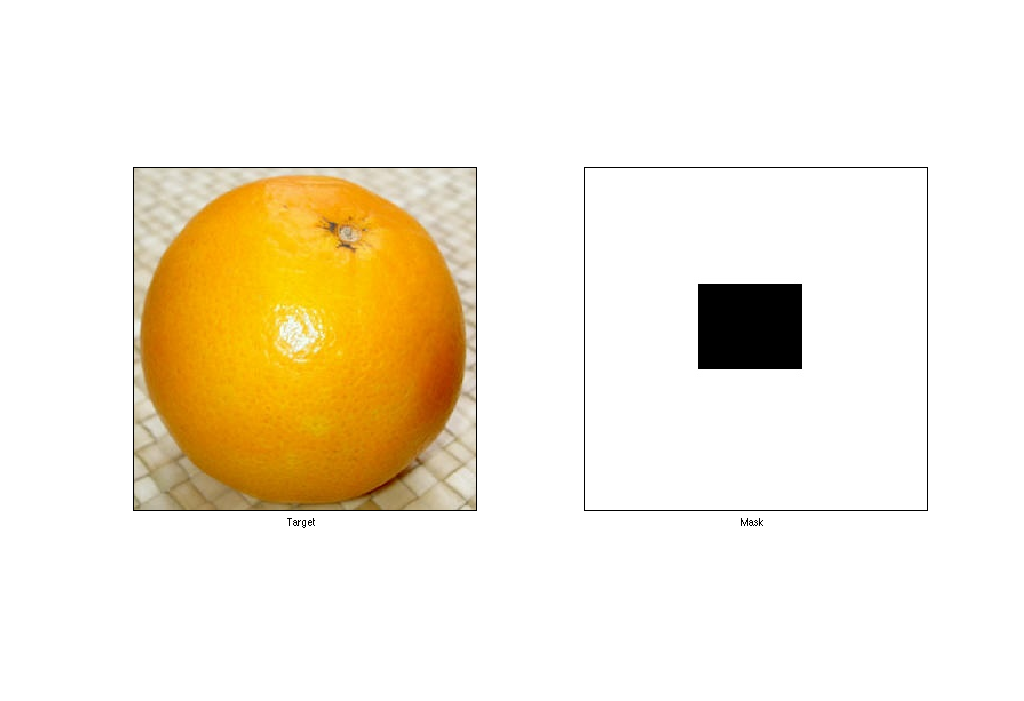
\includegraphics[width=\textwidth]{../../outputs/p4/highlight_removal/input}
    \end{subfigure}
    \caption{Visualization of Input images: Target Image is an image of an orange exhibiting a specular spot (left) and the corresponding mask (right) that encloses the highlight}
    \label{fig:highlight_removal_input}       
\end{figure}


\begin{figure}[H]
    \centering
    \begin{subfigure}{1.0\textwidth}
        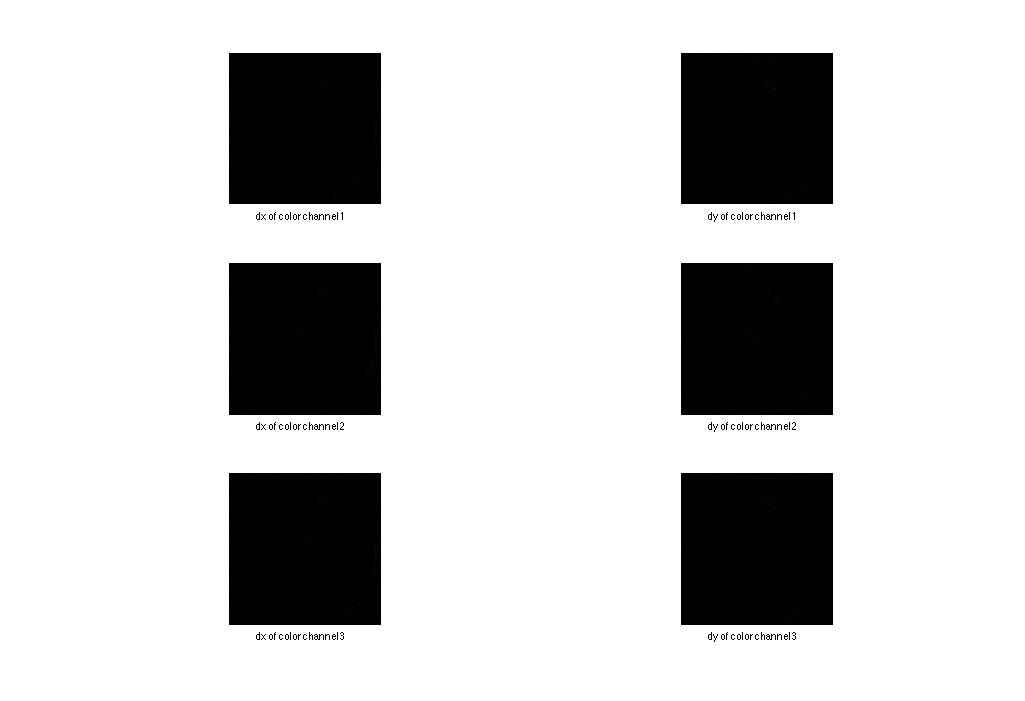
\includegraphics[width=\textwidth]{../../outputs/p4/highlight_removal/gradients4colorchannels}
    \end{subfigure}
    \caption{Visualization of Gradient field along $dx$ and $dy$ resulting from the gradient mixing gradient field applied on each color channel separately.}
    \label{fig:highlight_removal_gradients}       
\end{figure}


\begin{figure}[H]
    \centering
    \begin{subfigure}{1.0\textwidth}
        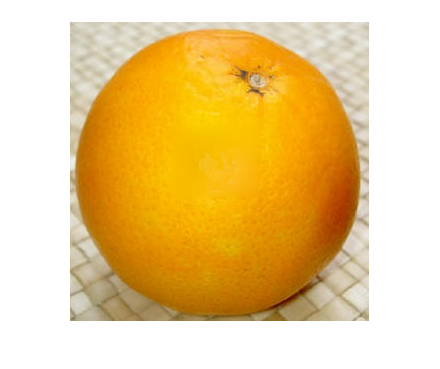
\includegraphics[width=\textwidth]{../../outputs/p4/highlight_removal/output_alphacompression}
    \end{subfigure}
    \caption{Output resulting from the gradient mixing method applied on our given input images using the gradient field as shown above.}
    \label{fig:highlight_removal_out_alphacompression}       
\end{figure}

\begin{figure}[H]
    \centering
    \begin{subfigure}{1.0\textwidth}
        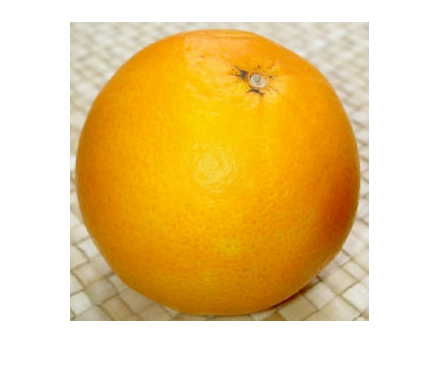
\includegraphics[width=\textwidth]{../../outputs/p4/highlight_removal/output_gammacompression}
    \end{subfigure}
    \caption{Output resulting from the gradient mixing method applied on our given input images using the gradient field as shown above.}
    \label{fig:highlight_removal_out_gammacompression}       
\end{figure}


\section{Image Segmentation}

In this part of the project I have implemented an interactive image segmentation tool using graph cut opimization.

\subsection{Sheep Example}

Selection foreground sheep, background grass and some hay in the background gives us quite nice segmentation results. \\

In the following the results from some experiments I performed. For the smoothness therm I used a gamma parameter value equal to $20$. In the \emph{outputs} folder are additional examples using different values for gamma. \\

Note that a user can modify the value of gamma which is determing the smoothness penalty in the file \emph{computeGraphSmoothness.m}. \

You can start a Matlab demo of my image segmentation code by running the script \emph{start4.m}. In order to run my image segmentation code on an arbitrary, user-specified image, you have to run the Matlab function \emph{imageSegmentation.m}. This function expects being provided by an input image - this image is supposed to be segmented into a foreground-and a background image. \\

When running this function, a user has to specify foreground-and background masks. When running my function, a GUI will pop up, allowing a user to specify this masked regions. Please follow the instructions given by the Matlab console, when the GUI is running. Type \emph{'f'} in order to select a foreground mask, type \emph{'b'} to specify a background mask in the image or enter \emph{'e'} to exit the mask selection process. \\

After the user has provided masking regions, the program will run by its own and computes the image segmentation. In addition it also will show some other helpful information: The user-specified masks, the probability images that a certain pixel belongs to the fore-or background, the mean colors of the fore-and background images, the smoothness term image and last, the segmentation of the image into a foreground and background image.

% input and selection
\begin{figure}[H]
    \centering
    \begin{subfigure}{0.45\textwidth}
        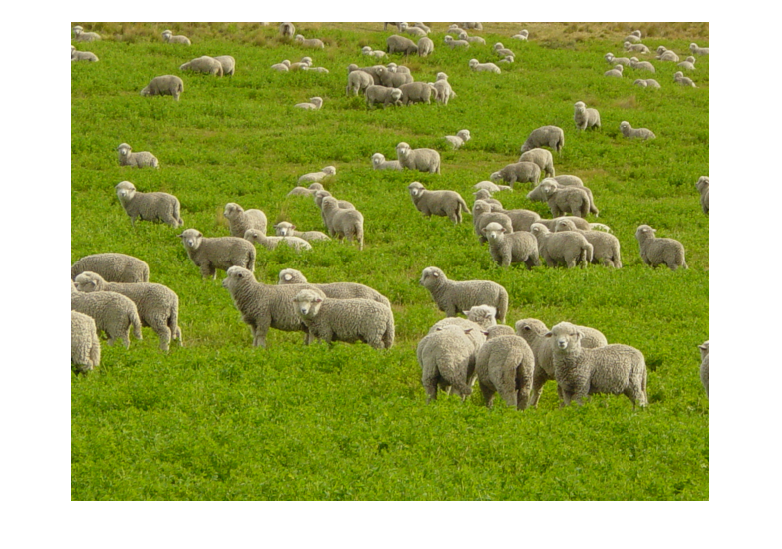
\includegraphics[width=\textwidth]{../../outputs/p4/image_segmentation/sheeps/input}
    \end{subfigure}
    ~
        \begin{subfigure}{0.45\textwidth}
        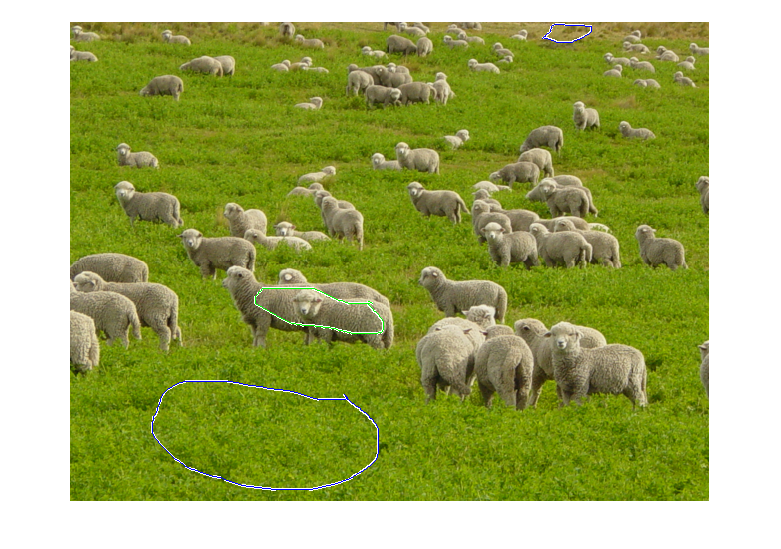
\includegraphics[width=\textwidth]{../../outputs/p4/image_segmentation/sheeps/selection}
    \end{subfigure}
    
    \caption{Used Input (left) and Selection provided by user (right) whereas a green selection indicates foreground and a blue selection indicates the background.}
    \label{fig:segmentation_sheeps_input_selection}       
\end{figure}

% masks
\begin{figure}[H]
    \centering
    \begin{subfigure}{1.0\textwidth}
        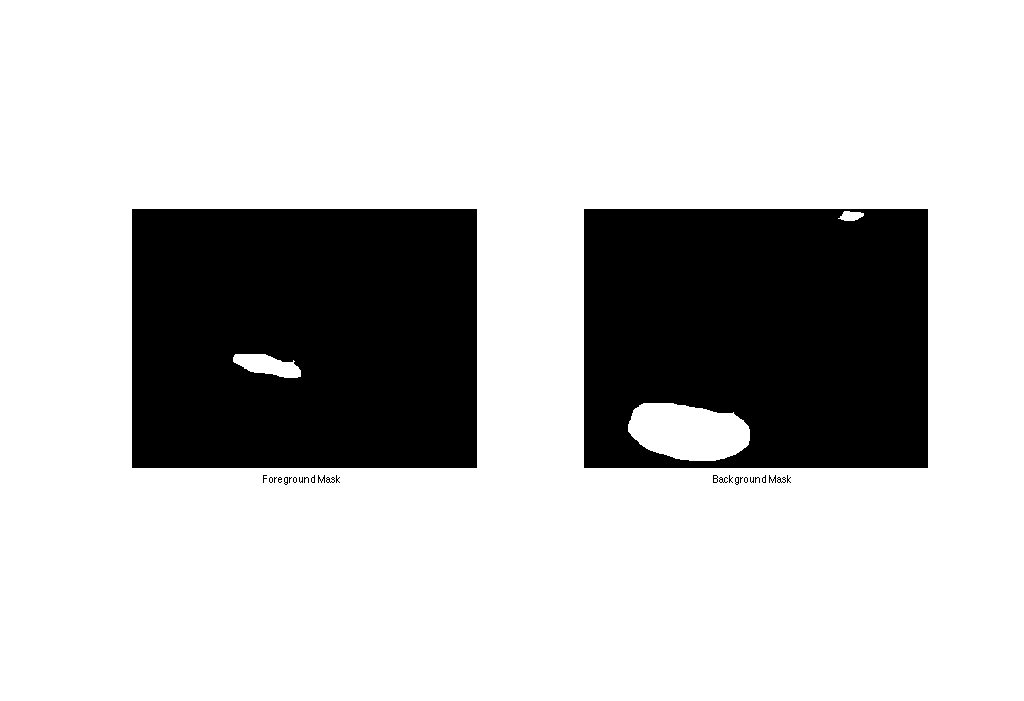
\includegraphics[width=\textwidth]{../../outputs/p4/image_segmentation/sheeps/masks}
    \end{subfigure}
    \caption{On the left the Foreground Mask and on the right the Background mask. For the foreground mask a white regions indicate that such a region should be interpreted as foreground. Similarly for the background mask.}
    \label{fig:segmentation_sheeps_masks}       
\end{figure}


% mean colors
\begin{figure}[H]
    \centering
    \begin{subfigure}{0.45\textwidth}
        
\includegraphics[width=\textwidth]{../../outputs/p4/image_segmentation/sheeps/mean_fg}
    \end{subfigure}
    ~
        \begin{subfigure}{0.45\textwidth}
        
\includegraphics[width=\textwidth]{../../outputs/p4/image_segmentation/sheeps/mean_bg}
    \end{subfigure}
    
    \caption{On the left the foreground mean colors and on the right the mean background colors.}
    \label{fig:segmentation_sheeps_mean_colors}       
\end{figure}


% probabilities
\begin{figure}[H]
    \centering
    \begin{subfigure}{0.45\textwidth}
        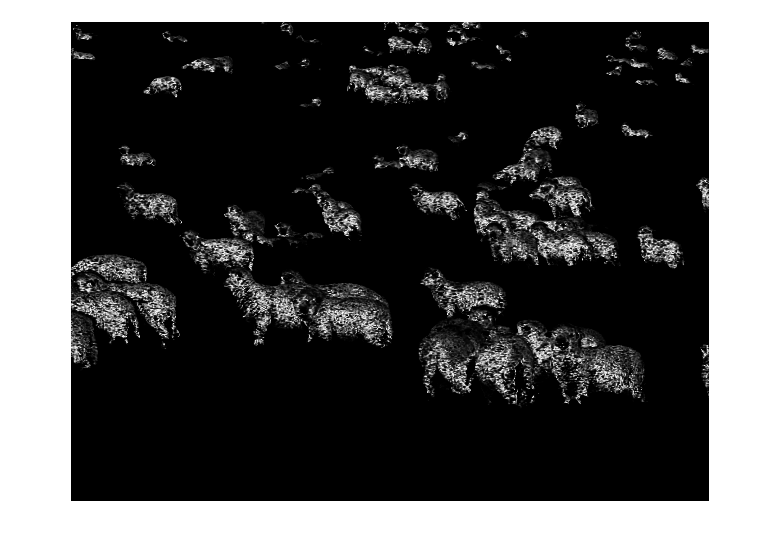
\includegraphics[width=\textwidth]{../../outputs/p4/image_segmentation/sheeps/prob_fg}
    \end{subfigure}
    ~
        \begin{subfigure}{0.45\textwidth}
        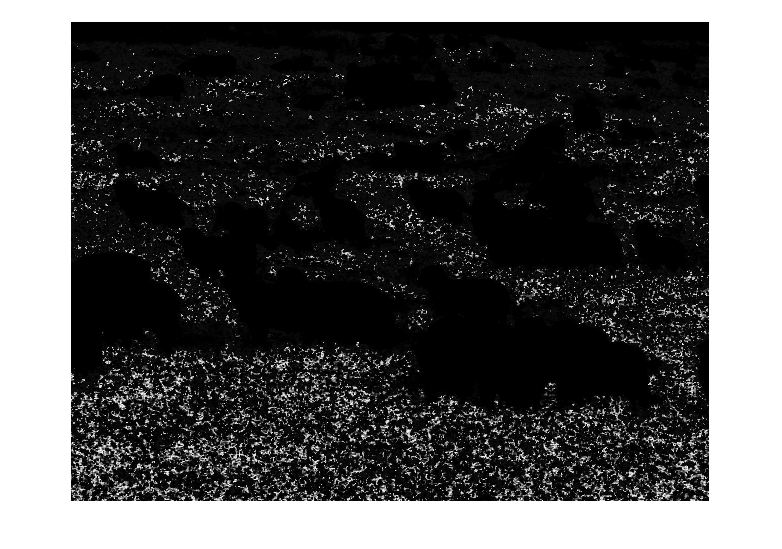
\includegraphics[width=\textwidth]{../../outputs/p4/image_segmentation/sheeps/prob_bg}
    \end{subfigure}
    
    \caption{On the left the probability a pixel belongs to the foreground and on the right the probability a pixel belongs to the background. The whiter the higher the probability is.}
    \label{fig:segmentation_sheeps_probabilities}       
\end{figure}

% smoothness
\begin{figure}[H]
    \centering
    \begin{subfigure}{1.0\textwidth}
        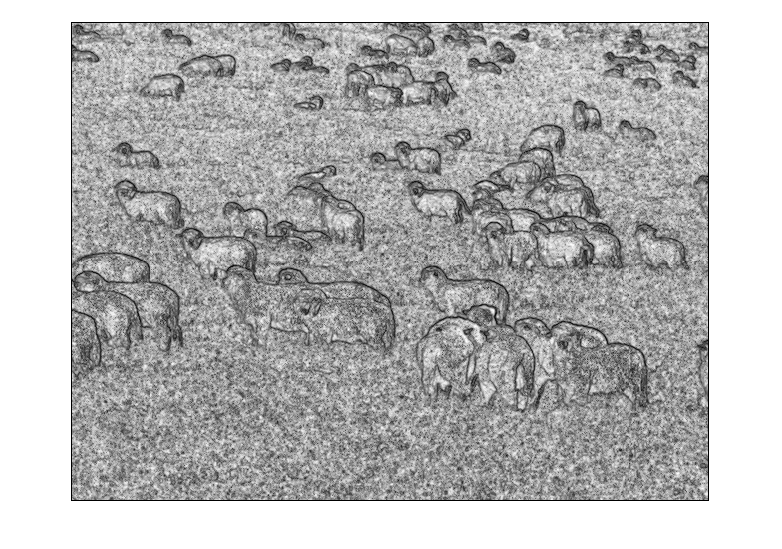
\includegraphics[width=\textwidth]{../../outputs/p4/image_segmentation/sheeps/smoothness}
    \end{subfigure}
    \caption{Illustration of the smoothness term.}
    \label{fig:segmentation_sheeps_smoothness}       
\end{figure}

% segmentation
\begin{figure}[H]
    \centering
    \begin{subfigure}{1.0\textwidth}
        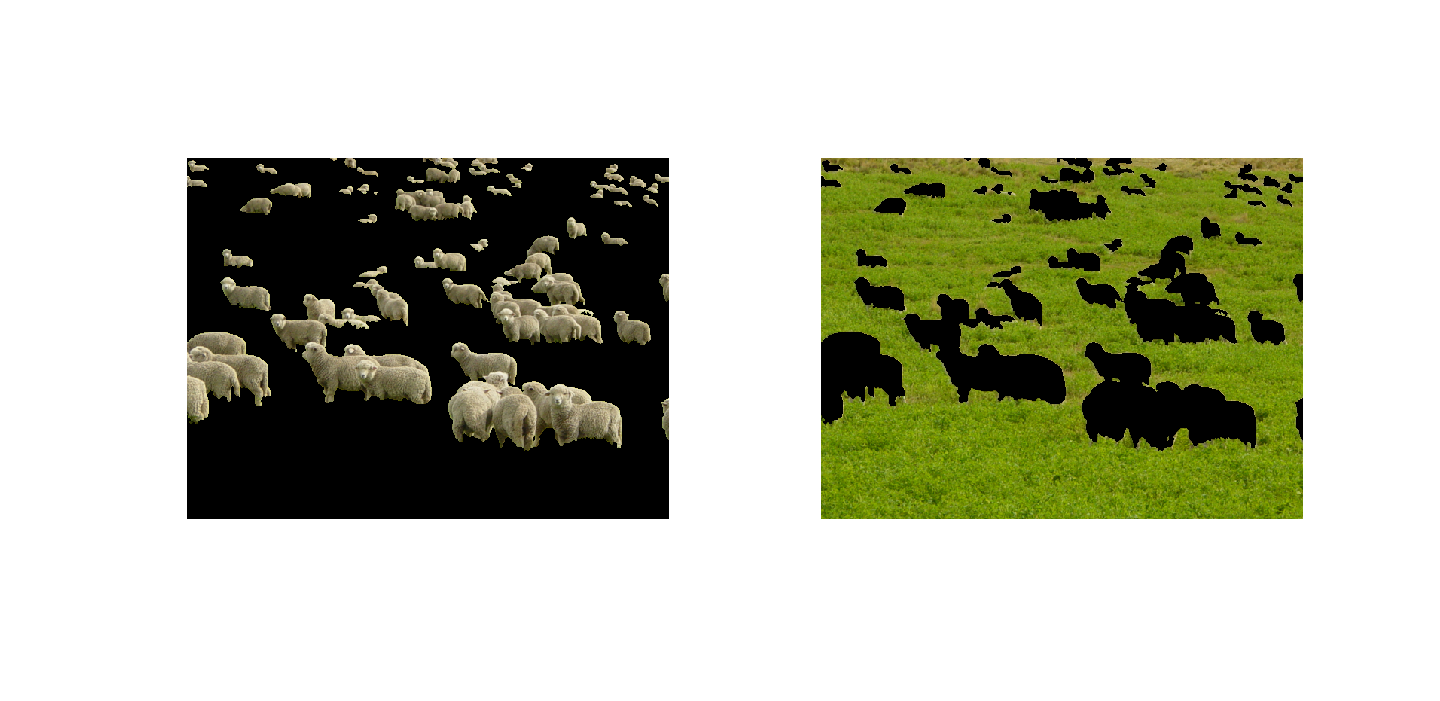
\includegraphics[width=\textwidth]{../../outputs/p4/image_segmentation/sheeps/segmentation}
    \end{subfigure}
    \caption{The segmentation of the image: On the left the Foreground image and on the right the background image}
    \label{fig:segmentation_sheeps_segmenation}       
\end{figure}


\subsection{Zebra Example}

Selection foreground sheep, background grass and some hay in the background gives us quite nice segmentation results.

% input and selection
\begin{figure}[H]
    \centering
    \begin{subfigure}{0.45\textwidth}
        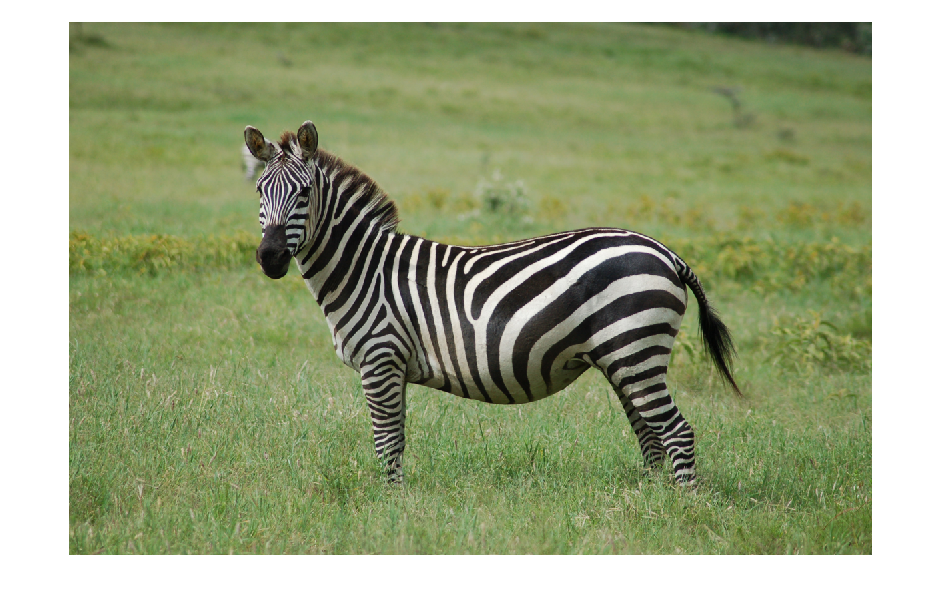
\includegraphics[width=\textwidth]{../../outputs/p4/image_segmentation/zebra/gamma20/input}
    \end{subfigure}
    ~
        \begin{subfigure}{0.45\textwidth}
        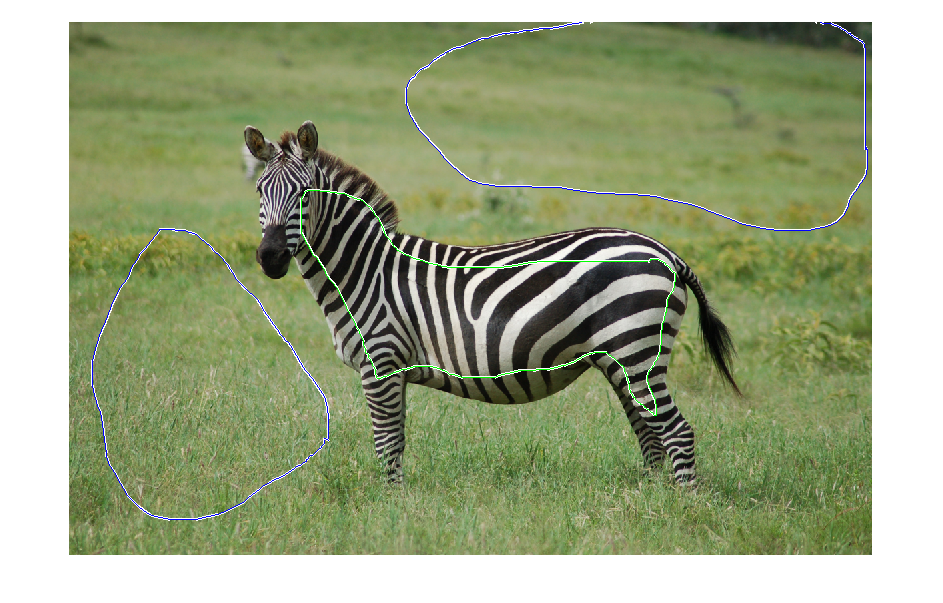
\includegraphics[width=\textwidth]{../../outputs/p4/image_segmentation/zebra/gamma20/selection}
    \end{subfigure}
    
    \caption{Used Input (left) and Selection provided by user (right) whereas a green selection indicates foreground and a blue selection indicates the background.}
    \label{fig:segmentation_zebra_input_selection}       
\end{figure}

% masks
\begin{figure}[H]
    \centering
    \begin{subfigure}{1.0\textwidth}
        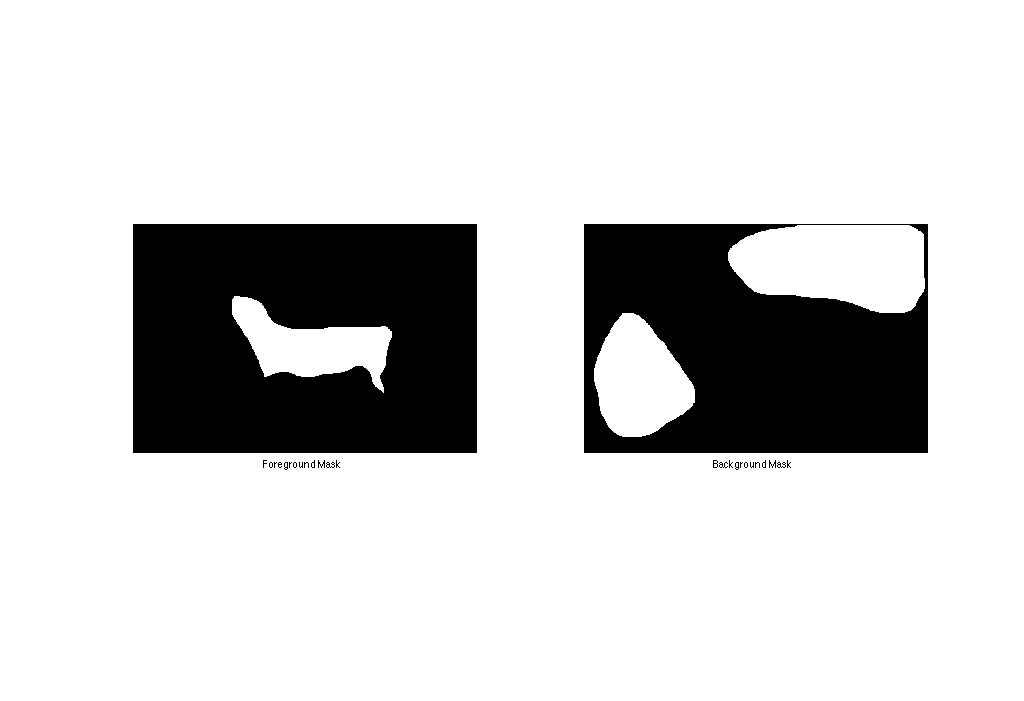
\includegraphics[width=\textwidth]{../../outputs/p4/image_segmentation/zebra/gamma20/masks}
    \end{subfigure}
    \caption{On the left the Foreground Mask and on the right the Background mask. For the foreground mask a white regions indicate that such a region should be interpreted as foreground. Similarly for the background mask.}
    \label{fig:segmentation_zebra_masks}       
\end{figure}


% mean colors
\begin{figure}[H]
    \centering
    \begin{subfigure}{0.45\textwidth}
        
\includegraphics[width=\textwidth]{../../outputs/p4/image_segmentation/zebra/gamma20/mean_fg}
    \end{subfigure}
    ~
        \begin{subfigure}{0.45\textwidth}
        
\includegraphics[width=\textwidth]{../../outputs/p4/image_segmentation/zebra/gamma20/mean_bg}
    \end{subfigure}
    
    \caption{On the left the foreground mean colors and on the right the mean background colors.}
    \label{fig:segmentation_zebra_mean_colors}       
\end{figure}


% probabilities
\begin{figure}[H]
    \centering
    \begin{subfigure}{0.45\textwidth}
        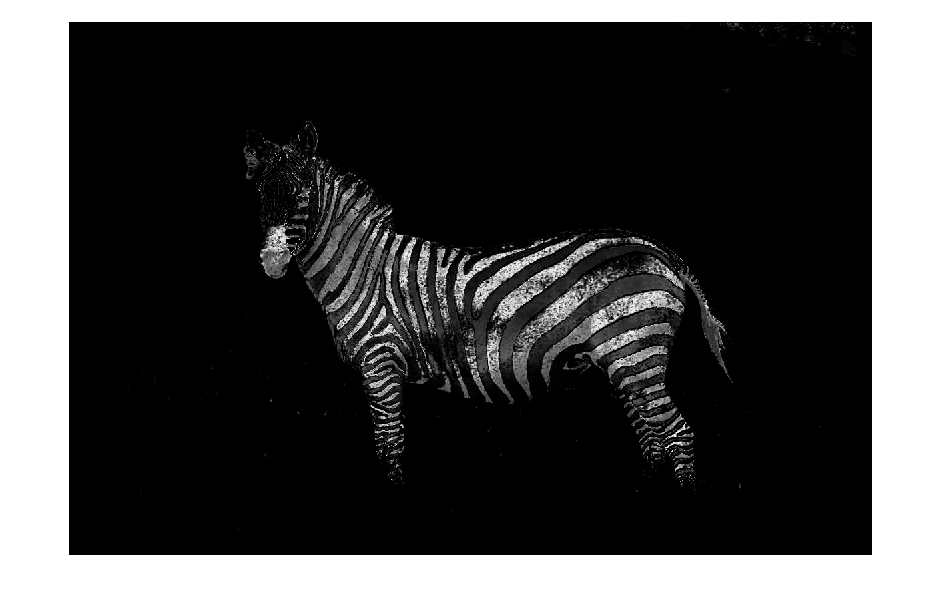
\includegraphics[width=\textwidth]{../../outputs/p4/image_segmentation/zebra/gamma20/prob_fg}
    \end{subfigure}
    ~
        \begin{subfigure}{0.45\textwidth}
        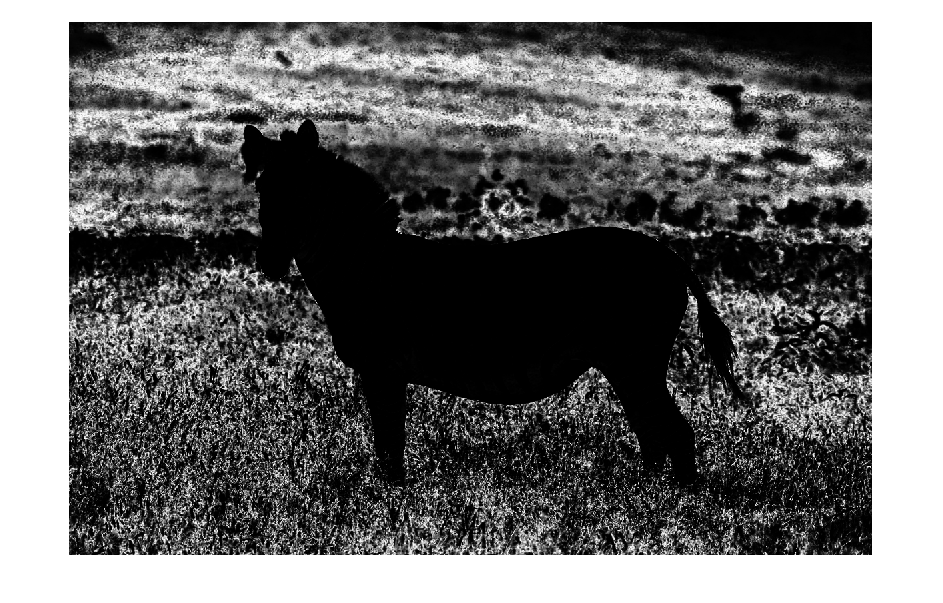
\includegraphics[width=\textwidth]{../../outputs/p4/image_segmentation/zebra/gamma20/prob_bg}
    \end{subfigure}
    
    \caption{On the left the probability a pixel belongs to the foreground and on the right the probability a pixel belongs to the background. The whiter the higher the probability is.}
    \label{fig:segmentation_zebra_probabilities}       
\end{figure}

% smoothness
\begin{figure}[H]
    \centering
    \begin{subfigure}{1.0\textwidth}
        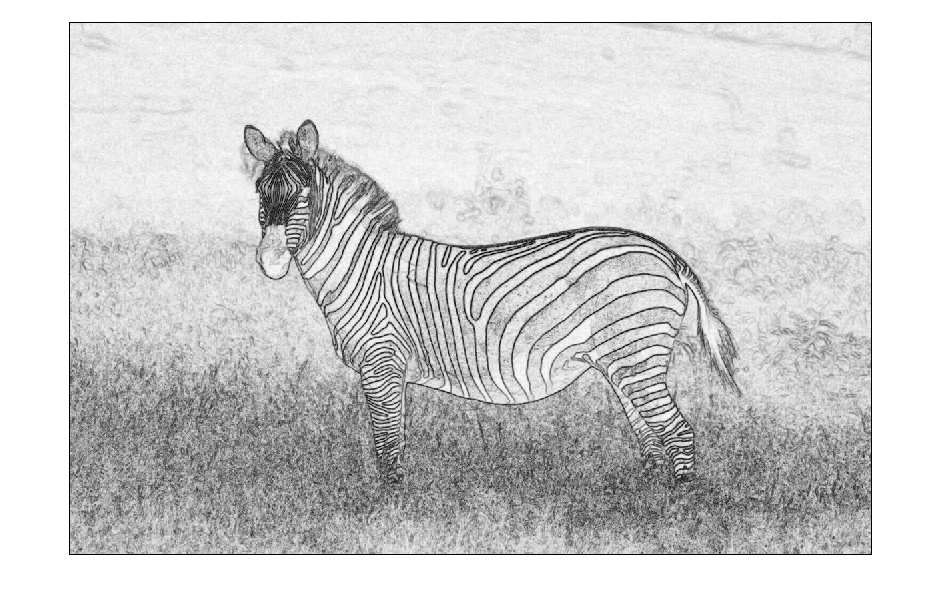
\includegraphics[width=\textwidth]{../../outputs/p4/image_segmentation/zebra/gamma20/smoothness}
    \end{subfigure}
    \caption{Illustration of the smoothness term.}
    \label{fig:segmentation_zebra_smoothness}       
\end{figure}

% segmentation
\begin{figure}[H]
    \centering
    \begin{subfigure}{1.0\textwidth}
        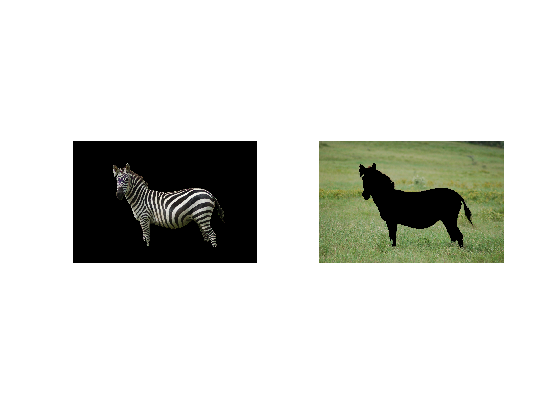
\includegraphics[width=\textwidth]{../../outputs/p4/image_segmentation/zebra/gamma20/segmentation}
    \end{subfigure}
    \caption{The segmentation of the image: On the left the Foreground image and on the right the background image}
    \label{fig:segmentation_zebra_segmenation}       
\end{figure}


\subsection{Second Zebra Example}

Selection foreground sheep, background grass and some hay in the background gives us quite nice segmentation results.

% input and selection
\begin{figure}[H]
    \centering
    \begin{subfigure}{0.45\textwidth}
        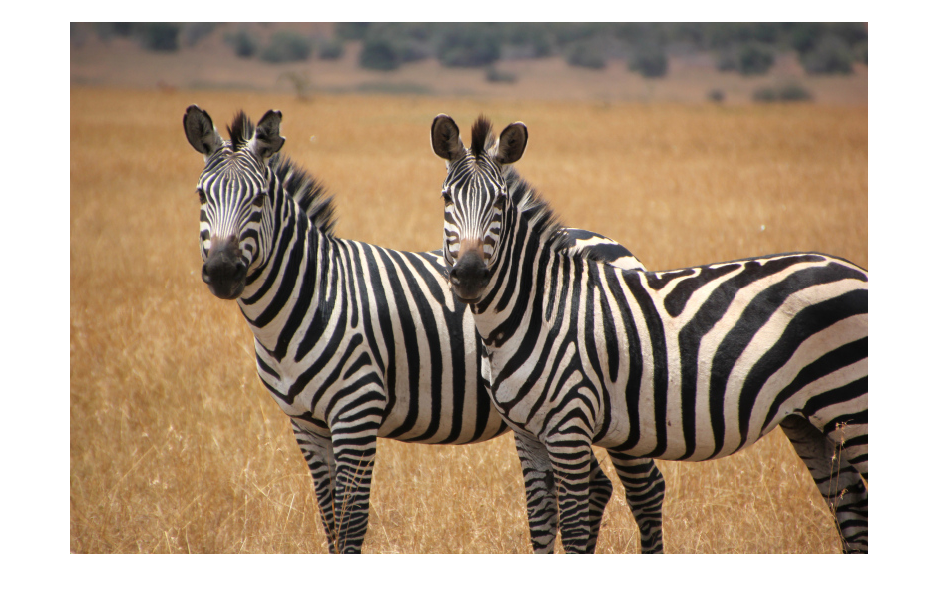
\includegraphics[width=\textwidth]{../../outputs/p4/image_segmentation/zebra2/input}
    \end{subfigure}
    ~
        \begin{subfigure}{0.45\textwidth}
        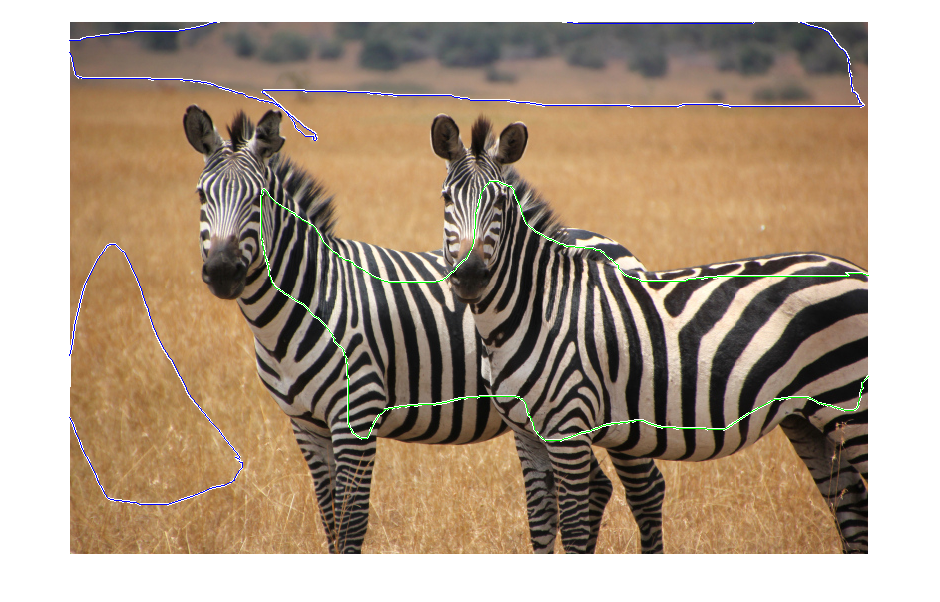
\includegraphics[width=\textwidth]{../../outputs/p4/image_segmentation/zebra2/selection}
    \end{subfigure}
    
    \caption{Used Input (left) and Selection provided by user (right) whereas a green selection indicates foreground and a blue selection indicates the background.}
    \label{fig:segmentation_zebra2_input_selection}       
\end{figure}

% masks
\begin{figure}[H]
    \centering
    \begin{subfigure}{1.0\textwidth}
        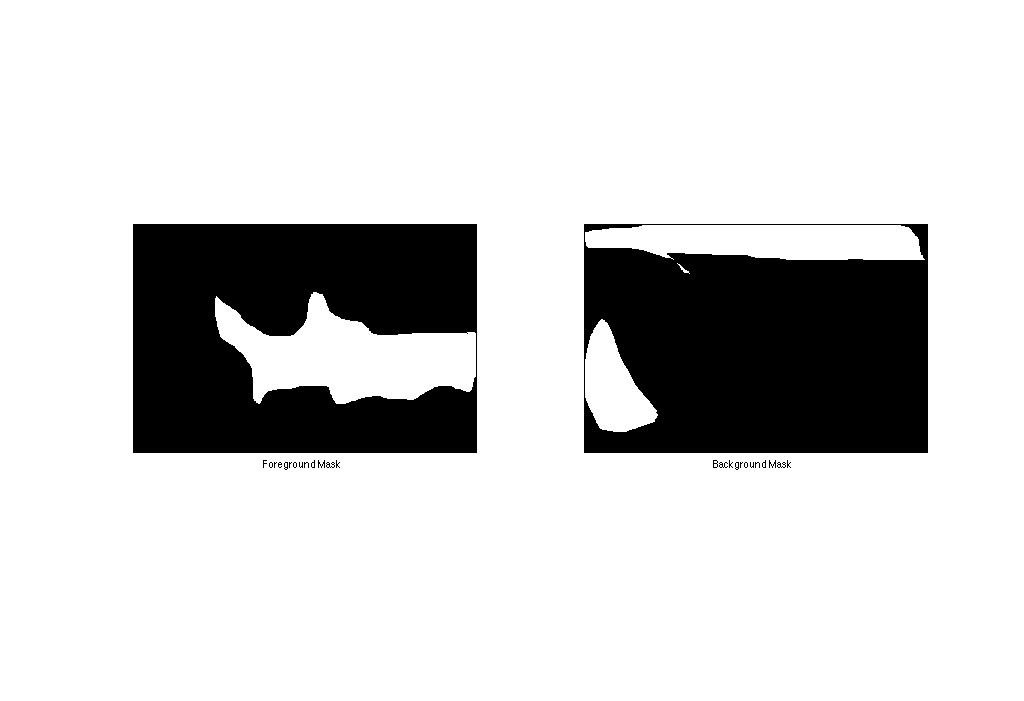
\includegraphics[width=\textwidth]{../../outputs/p4/image_segmentation/zebra2/masks}
    \end{subfigure}
    \caption{On the left the Foreground Mask and on the right the Background mask. For the foreground mask a white regions indicate that such a region should be interpreted as foreground. Similarly for the background mask.}
    \label{fig:segmentation_zebra2_masks}       
\end{figure}


% mean colors
\begin{figure}[H]
    \centering
    \begin{subfigure}{0.45\textwidth}
        
\includegraphics[width=\textwidth]{../../outputs/p4/image_segmentation/zebra2/mean_fg}
    \end{subfigure}
    ~
        \begin{subfigure}{0.45\textwidth}
        
\includegraphics[width=\textwidth]{../../outputs/p4/image_segmentation/zebra2/mean_bg}
    \end{subfigure}
    
    \caption{On the left the foreground mean colors and on the right the mean background colors.}
    \label{fig:segmentation_zebra2_mean_colors}       
\end{figure}


% probabilities
\begin{figure}[H]
    \centering
    \begin{subfigure}{0.45\textwidth}
        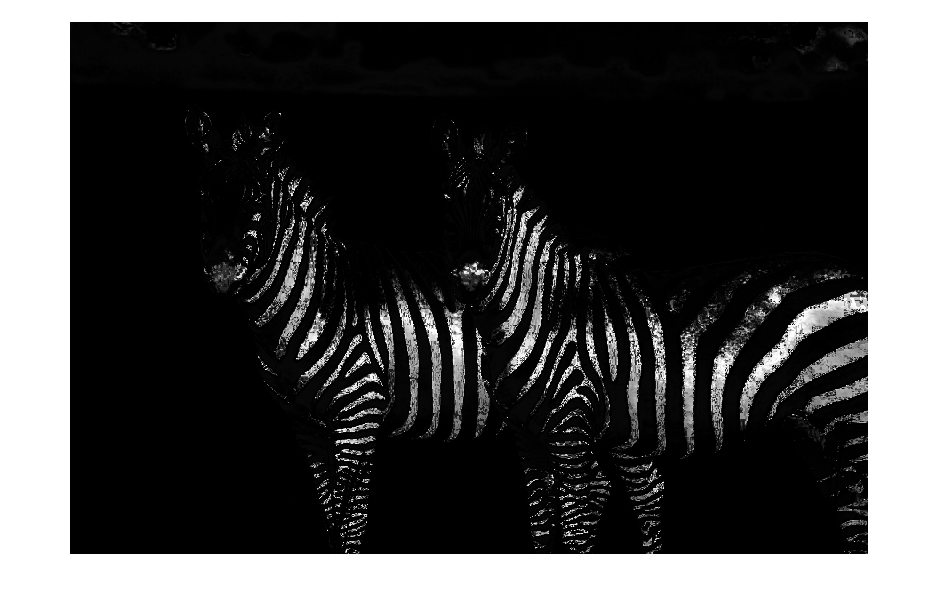
\includegraphics[width=\textwidth]{../../outputs/p4/image_segmentation/zebra2/prob_fg}
    \end{subfigure}
    ~
        \begin{subfigure}{0.45\textwidth}
        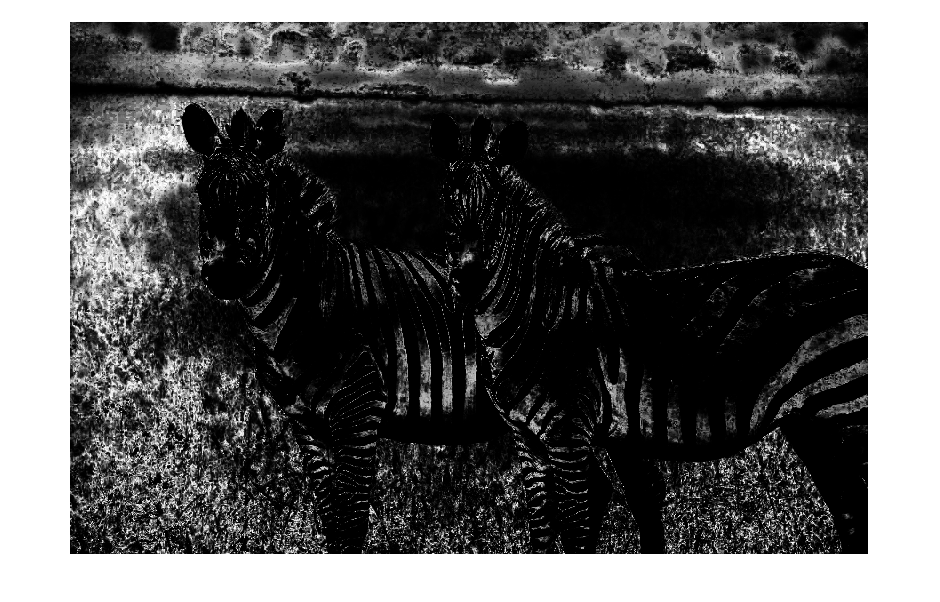
\includegraphics[width=\textwidth]{../../outputs/p4/image_segmentation/zebra2/prob_bg}
    \end{subfigure}
    
    \caption{On the left the probability a pixel belongs to the foreground and on the right the probability a pixel belongs to the background. The whiter the higher the probability is.}
    \label{fig:segmentation_zebra2_probabilities}       
\end{figure}

% smoothness
\begin{figure}[H]
    \centering
    \begin{subfigure}{1.0\textwidth}
        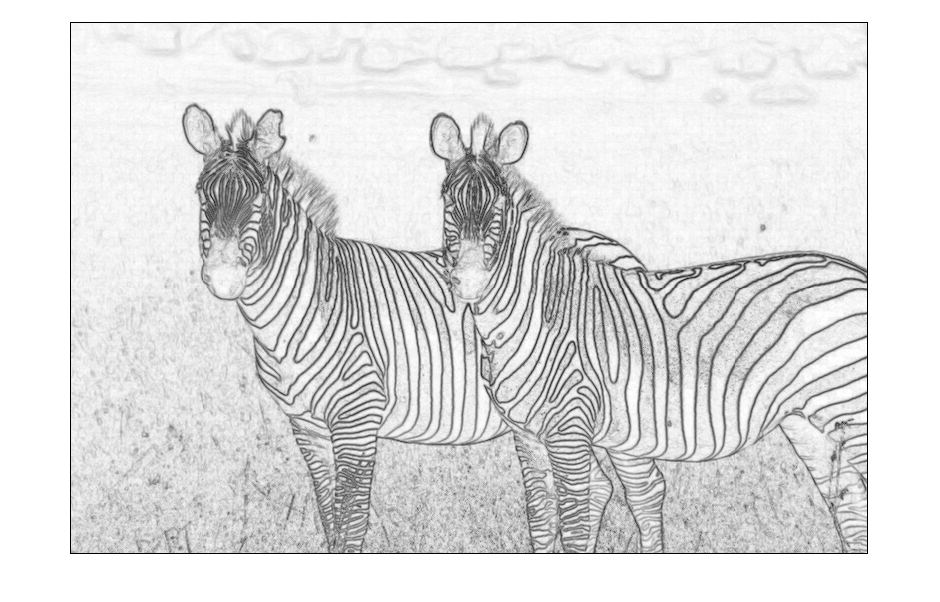
\includegraphics[width=\textwidth]{../../outputs/p4/image_segmentation/zebra2/smoothness}
    \end{subfigure}
    \caption{Illustration of the smoothness term.}
    \label{fig:segmentation_zebra2_smoothness}       
\end{figure}

% segmentation
\begin{figure}[H]
    \centering
    \begin{subfigure}{1.0\textwidth}
        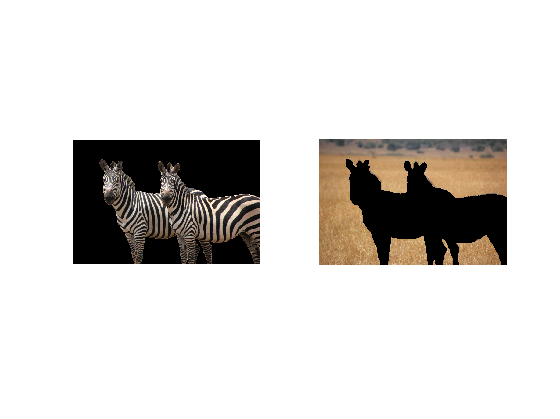
\includegraphics[width=\textwidth]{../../outputs/p4/image_segmentation/zebra2/segmentation}
    \end{subfigure}
    \caption{The segmentation of the image: On the left the Foreground image and on the right the background image}
    \label{fig:segmentation_zebra2_segmenation}       
\end{figure}



\end{document}